\documentclass[11pt]{article}% uses letterpaper by default

%---------- Uncomment one of them ------------------------------
\usepackage[includeheadfoot, top=1in, bottom=1in, hmargin=1in]{geometry}

% \usepackage[a5paper, landscape, twocolumn, twoside,
%    left=2cm, hmarginratio=2:1, includemp, marginparwidth=43pt, 
%    bottom=1cm, foot=.7cm, includefoot, textheight=11cm, heightrounded,
%    columnsep=1cm, dvips,  verbose]{geometry}
%---------------------------------------------------------------
\usepackage{fancyhdr}
\renewcommand{\footrulewidth}{0.4pt}% default is 0pt
\usepackage{verbatim}
\usepackage{url}
\usepackage{cancel}
\pagestyle{fancy}
\usepackage{graphicx}
\usepackage{setspace}
\singlespacing
%\doublespacing
%\onehalfspacing
\usepackage{varwidth}

\newcommand{\degrees}{\ensuremath{^\circ}}
\newcommand{\arcmin}{\ensuremath{'}}
\newcommand{\arcsec}{\ensuremath{"}}
\newcommand{\hours}{\ensuremath{^\mathrm{h}}}
\newcommand{\minutes}{\ensuremath{^\mathrm{m}}}
\newcommand{\seconds}{\ensuremath{^\mathrm{s}}}

\newcommand{\s}[0]{\phantom{i}} %sets up \s command
\newcommand{\m}[0]{\phantom{abcde}} %sets up \m command
\providecommand{\e}[1]{\ensuremath{\times 10^{#1}}} %sets up \e command
\setlength{\parindent}{0.2in} %new paragraph indent
\usepackage{indentfirst} % indent the first paragraph of a section
\usepackage{amsmath,amssymb}
\usepackage{enumitem}

\lhead{Astronomy Lab II}
\rhead{Fall 2024}
\lfoot{Porter}
\rfoot{Wed 6-9pm}
\cfoot{\thepage}

%\newcommand{\exercisename}{7}
\begin{document}

\begin{center}
\huge{Lab 7: Dark Matter}\\ \medskip \Large{October 30, 2024}
\end{center}

%%%%%%%%%%%%%%%%%%%%%%% INTRODUCTION %%%%%%%%%%%%%%%%%%%%%%%
\section{Introduction}
% Note to future readers of this tex doc - midway through the lab, the students took a tour of the 10th-floor Columbia XENON experiment to learn about direct detection of dark matter 

\noindent
Over the past few weeks, we've spent a lot of time talking about \emph{light}: we've talked about telescopes and spectrometers, and how these tools can help us study stars and galaxies. However, not all of the matter in the Universe emits light -- indeed, \emph{most} of the matter in the Universe doesn't emit light! We call this non-radiating matter \textbf{``dark matter''}. While we cannot see dark matter, we can infer the presence of dark matter from its gravitational influence on luminous matter. In this lab, we'll look at some of the most convincing astrophysical evidence for the existence of dark matter: \textit{galactic rotation curves}.

\medskip \noindent
The \textbf{rotation curve} of a spiral galaxy is a measurement of how fast the galaxy rotates at different distances from its center.  Galaxies don't rotate as solid bodies (like records on a turntable or merry-go-rounds); rather, they rotate \textit{differentially}, with the inner parts moving faster than the outer parts. In this lab, you will use Newton's Law of Gravitation to investigate this differential rotation and to learn how rotation curves can be used to probe the dark matter content of large galaxies.

\begin{enumerate}
\setcounter{enumi}{0}
    \item Before beginning this lab, what have you previously known about dark matter? If necessary, think back to previous labs or lectures.
    
\end{enumerate}

%%%%%%%%%%%%%%%%%%%%%%% SOLAR SYSTEM %%%%%%%%%%%%%%%%%%%%%%%
\section{Differential Rotation in the Solar System}
\noindent
In space, almost everything is orbiting something: the moon orbits the Earth, the Earth orbits the Sun, the Sun orbits the center of the Milky Way, and so forth. All of this motion is due to the force of \emph{gravity}, which pulls massive objects together. Newton's Law of Gravitation tells us that
\begin{equation}
F = \frac{G M_1 M_2}{r^2},
\end{equation}
or that the gravitational force ($F$, usually given units of \emph{Newtons}, or $\rm kg \, m/s^2$) between two bodies is proportional to the individual masses of the bodies ($M_1$ and $M_2$) and \emph{inversely} proportional to the square of their separation distance ($r$); the gravitational force is bigger when the two bodies are more massive and closer together. The proportionality constant, $G$ (sometimes called Newton's constant), has the weird value $6.67 \times 10^{-20} \, {\rm km^3/kg/s^2}$ -- these units are ugly, but as long as you keep your masses in kilograms, your distances in kilometers, and your times in seconds, everything should work out.


When under the influence of their mutual gravitational attraction, masses $M_1$ and $M_2$ both orbit their common \emph{center of mass}. When more complicated mass distributions are involved (i.e., situations with many orbiting bodies, as in the Solar System or the Milky Way), an object's orbital properties are influenced by  \emph{all} the mass within its own orbit. For example, the gravitational force on Earth is, properly,
\begin{equation}
F = \frac{G M_{\textrm{Earth}} \times (M_{\odot} + M_{\textrm{Mercury}} + M_{\textrm{Venus}})}{r^2};
\end{equation}
that is, the Earth's orbit is influenced by the masses of the Sun ($M_\odot$), Mercury, \emph{and} Venus -- the three bodies within Earth's orbit. Here, $r$ is the distance between Earth and the \emph{center of mass} of all four of these objects. Importantly, however, the Sun is so much more massive than anything else in the Solar System, so we can ignore the contributions of the other planets when we compute the gravitational force on Earth:
\begin{equation}
F = \frac{G M_{\textrm{Earth}} \times M_{\odot}}{r^2}.
\end{equation}
For an arbitrary planet orbiting an arbitrary star, this generalizes to
\begin{equation} \label{eq:grav}
F = \frac{G M_{\textrm{planet}} \times M_{\textrm{star}}}{r^2}.
\end{equation}

In our Solar System, the planets move on very nearly \emph{circular} orbits. The force on an object in a circular orbit is described by the equation:
\begin{equation} \label{eq:CF}
F = \frac{M v^2}{r},
\end{equation}
where $M$ is the orbiting body's mass, $v$ is its velocity, and $r$ is the radius of its orbit. If the force of gravity is what's causing the planets to orbit the Sun, then a little bit of algebra will tell us how the velocity of a planet is related to its distance from the Sun.

\textbf{Complete the following in your lab write-up}:

\begin{enumerate}
\setcounter{enumi}{1}
    \item The force of gravity on an orbiting body must equal its ``centripetal'' (or center-seeking) force, given by equation \ref{eq:CF}. Consider a planet (of mass $M_{\textrm{planet}}$) orbiting the Sun (with mass $M_\odot$). Set equations \ref{eq:grav} and \ref{eq:CF} equal to one other and solve for $v$ in terms of $M_{\odot}$, $G$, and $r$. Show all steps.
    
    \item We now have a theoretical prediction for the velocity of a planet orbiting the Sun.
    \begin{enumerate}
        \item Make a table with two columns and a row for each planet in the Solar System. The first column is for the planet's name and the second column is for the planet's orbital velocity. 
        
        \item Calculate the orbital velocity (in \textbf{km/s}) of each planet around the Sun by using your equation from Problem 1. For $r$, use the semimajor axes given in Table 1, but watch your units ($1 \, {\rm AU} = 1.50 \times 10^8 \, {\rm km}$)! For the mass of the Sun, use $M_\odot = 1.99 \times 10^{30} \, {\rm kg}$. (\emph{Hint}: it may be helpful to use Excel's or Google Sheets' Formula capabilities to quickly populate your table, but you must first make sure that all your units are consistent)
    \end{enumerate}
    
    \item Using the values in \emph{your} table, plot the theoretical \textbf{rotation curve} for our Solar System -- that is, plot the orbital velocity (in km/s) vs. the semimajor axis (in AU) for each planet. 
    
    \item Using the \emph{measured} values for average orbital velocity in Table 1, plot the \emph{actual} rotation curve (in km/s vs. AU). Does your theoretical rotation curve resemble the actual rotation curve? In other words, does the equation you derived in Problem 1 agree with the observed data?
\end{enumerate}

\begin{figure}[h!] \label{tab:planets}
\center
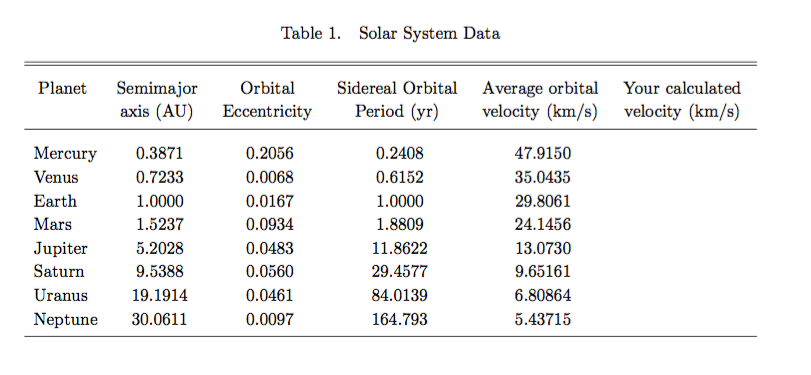
\includegraphics[scale=0.55]{Images/table1.png}
\label{table1}
\end{figure}


%%%%%%%%%%%%%%%%%%%%%%% ROTATION CURVES %%%%%%%%%%%%%%%%%%%%%%%
\break
\section{Differential Rotation in a Galaxy}

\noindent
In the last section, we used our knowledge of masses and distances in the Solar System to predict the orbital velocities of the planets. For entire galaxies, obtaining masses is tricky, but we can use the same principle as Equation 2: since the orbital properties of a star circling around the center of a galaxy depend on \emph{all} the mass contained within the star's orbit, we can use these orbits to deduce the galaxy's mass. 

Figure \ref{fig:rotcurve} shows a measured rotation curve for the spiral galaxy NGC 2742, observed nearly edge-on. Positive values of radial velocity indicate that stars are moving away from us, while negative radial velocities indicate that stars are moving towards us. Negative radius values are just used to indicate the opposite side of the galaxy from the positive radius values. 

\begin{figure}[h!]
\center
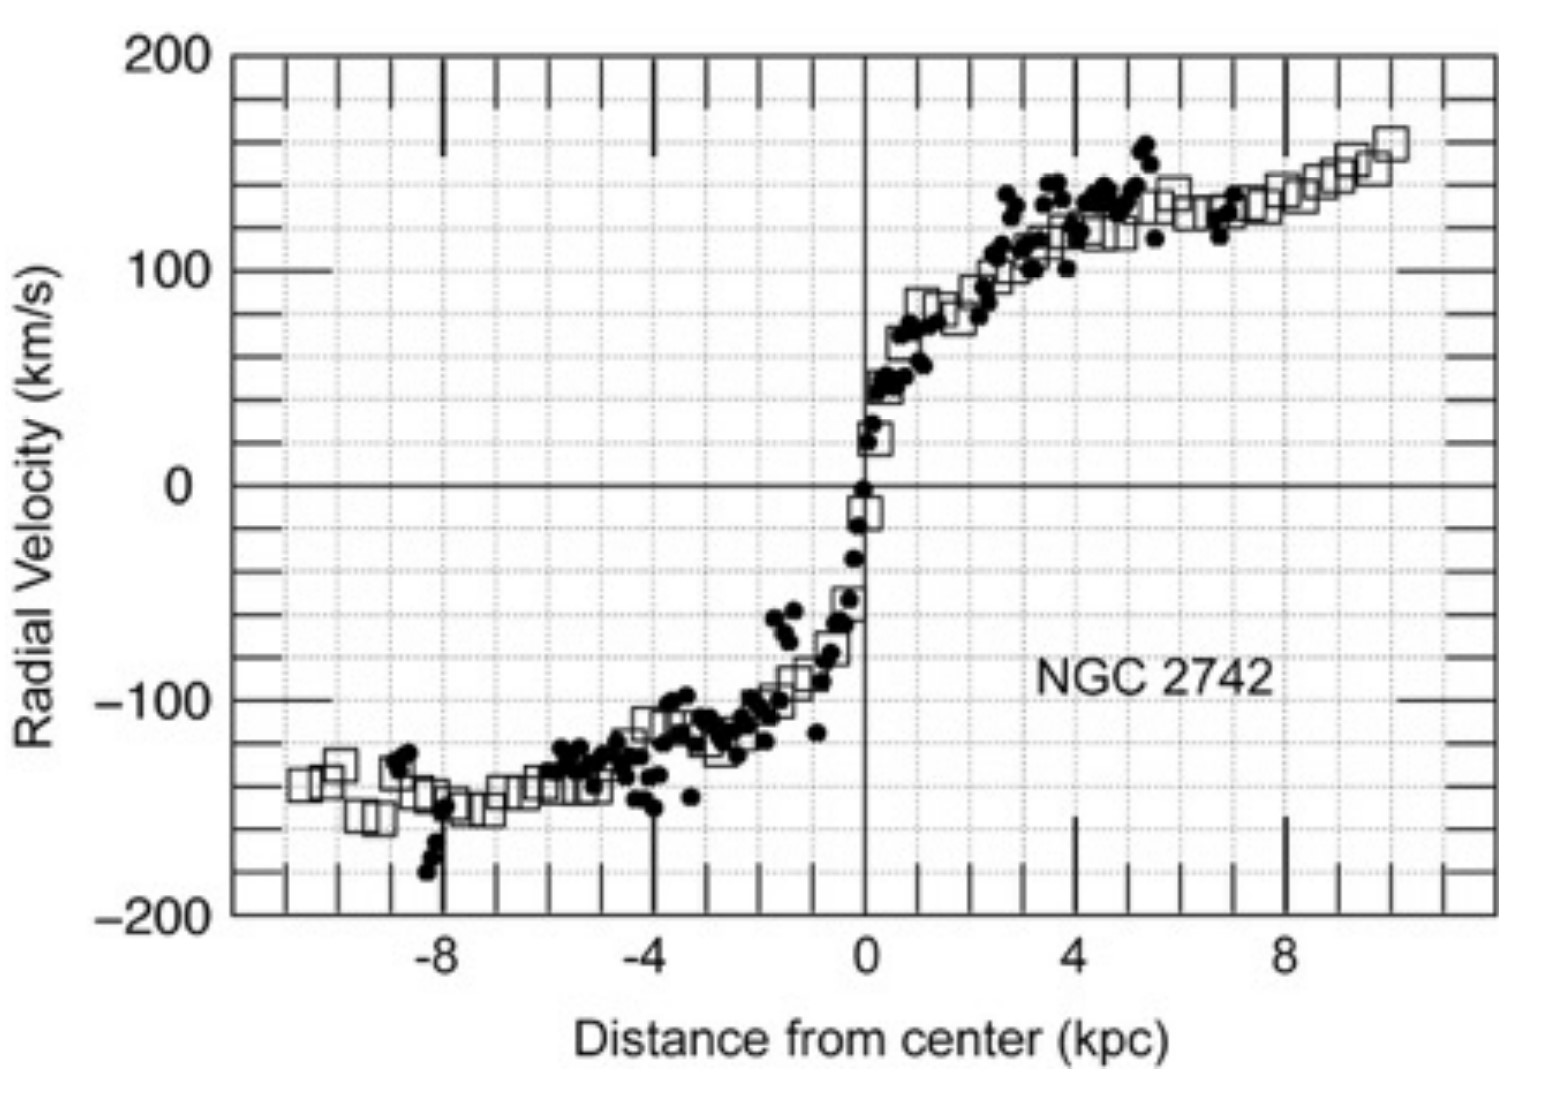
\includegraphics[scale=0.6]{Images/rotation curve 2742.jpg}
\caption{The rotation curve of NGC 2742.}
\label{fig:rotcurve}
\end{figure}

\begin{enumerate}
\setcounter{enumi}{5}

\item Draw a table in your lab write-up with 5 columns: Radius (in units of kpc), Rotational Velocity (in units of km/s), Gravitational Mass (in units of $M_{\odot}$), Luminosity (in units of $L_{\odot}$), and Luminous Mass (in units of $M_{\odot}$).

\item Select 7 evenly spaced radii from Figure \ref{fig:rotcurve} -- either all positive or all negative -- and record them in your table.

\item Use Figure \ref{fig:rotcurve} to measure the radial velocity at each of your radii. Record these velocities in your table.

\item Take the equation you derived in Problem 2 and rearrange it to isolate mass -- that is, put mass on the left-hand side of the equation and leave the velocity, orbital radius, and $G$ on the right-hand side. Show all steps. Recall that this mass is the \emph{total} mass enclosed by the orbit.

\item Find the amount of galactic mass enclosed within each of the radii you chose by plugging the numbers in your table into the equation you just derived. Record these (very big) values in your table under ``gravitational mass.'' Watch your units ($1 \, {\rm kpc} = 3.09 \times 10^{16} \, {\rm km}$)!  If you haven't done so already, convert your masses to units of \emph{solar mass} ($1 \, M_\odot = 1.99 \times 10^{30} \, {\rm kg}$).
\end{enumerate}

\noindent
Congrats -- you've just weighed a galaxy! By looking at stellar orbits and thinking about gravity, we've deduced that NGC 2742 has a mass equivalent to that of billions and billions of stars. But, is all this mass actually due to stars? Let's compare the mass of NGC 2742 to the \emph{amount of light} that the galaxy is producing, since the light comes from the stars and gas that the galaxy contains.  Figure \ref{fig:luminosity} shows the amount of galactic light emitted within different radii. 

\medskip \noindent
The comparison we're going to make is easier for some galaxies than others. It's tricky to figure out how much light is coming from a more ``edge-on'' spiral galaxy, since much of the light will be blocked by dust. Towards the other extreme, when we look at a spiral galaxy ``face-on,'' we see almost all of its light, but it's harder to accurately determine the galaxy's rotational velocity -- if the motion is perpendicular to our line of sight, we can't use redshifts or blueshifts to infer velocities. Thus, to get the best rotation curves and the best luminosity measurements, we need to observe galaxies in the happy medium between edge-on and face-on.


\begin{figure}[h!]
\center
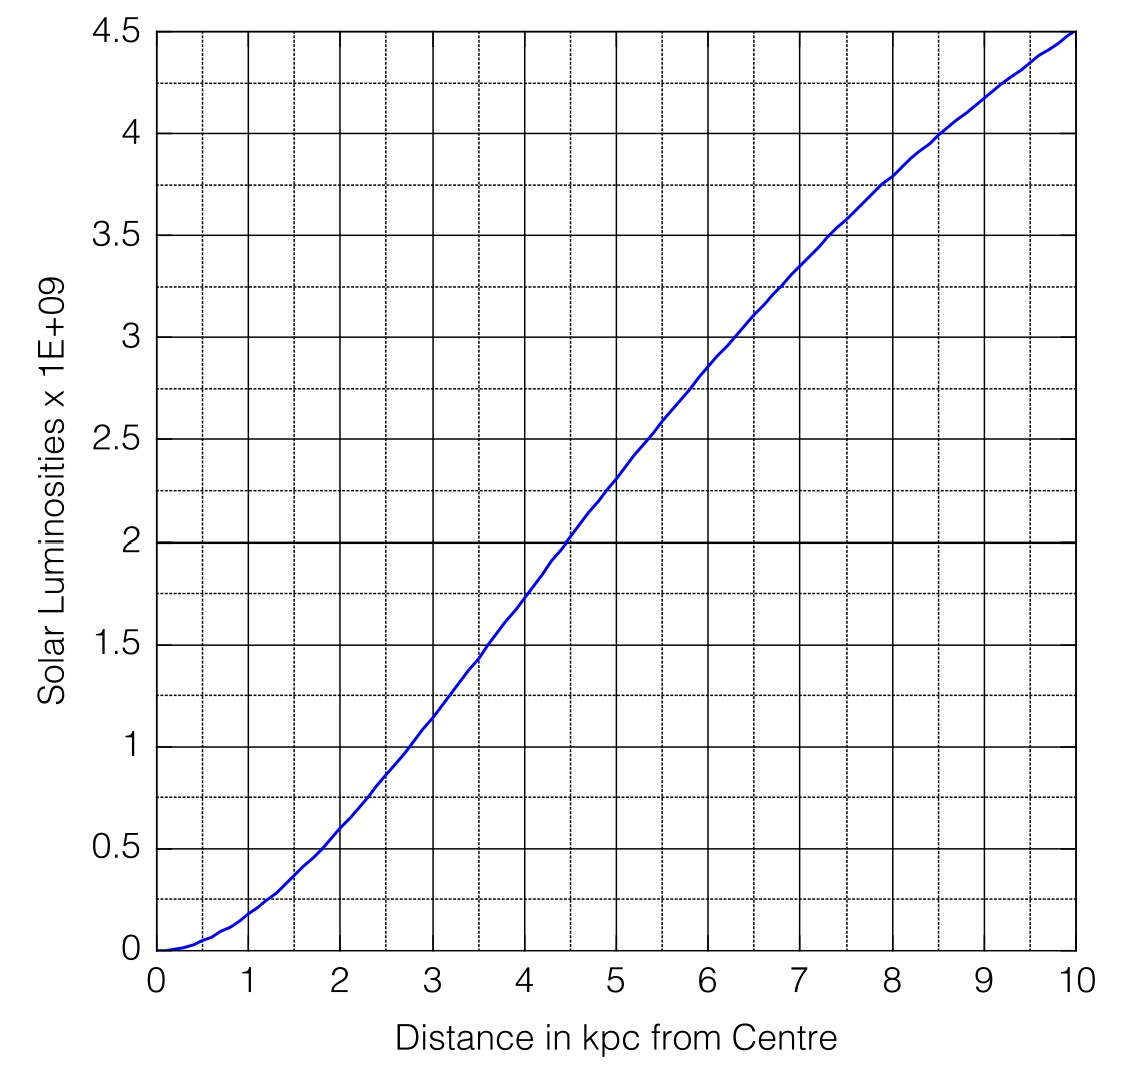
\includegraphics[scale=0.6]{Images/light curve 2742.jpg}
\caption{The amount of light emitted from inside a given radius in NGC 2742.}
\label{fig:luminosity}
\end{figure}

\begin{enumerate}
\setcounter{enumi}{10}

\item Refer back to your table with the properties of NGC 2742. At the same radii that you chose before, use Figure \ref{fig:luminosity} to determine the luminosity of the galaxy within that radius; record these values in your table (under the ``Luminosity'' column). (The `e' in the luminosity axis label in Figure \ref{fig:luminosity} indicates a power of ten: each of the values on the vertical axis should be multiplied by $10^9$)

\item The luminosity that we read off of Figure \ref{fig:luminosity} is largely contributed by a few young, bright stars with masses slightly greater than that of our Sun; as such, this plot is not a perfect tracer of the luminous matter in NGC 2742, since the galaxy likely contains many, many more low-mass, low-luminosity stars than big bright stars. To account for this, let's assume that the galaxy gains one unit of solar luminosity for every two solar masses of galactic matter. Using this, calculate how much mass should be present in NGC 2742 (within each radius) based on how much light we see. Record your values in the table under ``Luminous Mass.''

\item \emph{On the same graph}, plot the gravitational mass vs. radius \emph{and} the luminous mass vs. radius. Note any differences between the two plots. How do you physically interpret these differences - what is \textit{physically} happening in this scenario?

\item Comment on the matter content of NGC 2742:
\begin{enumerate}
    \item What percentage of the galaxy's total mass is \emph{luminous}? What percent cannot be accounted for by the light that we see?
    
    \item How much ``dark matter'' is in NGC 2742?
\end{enumerate}
 
\end{enumerate}

%%%%%%%%%%%%%%%%%%%%%%% CONCLUSIONS %%%%%%%%%%%%%%%%%%%%%%%
\section{Wrapping things up}
\begin{enumerate}
\setcounter{enumi}{14}

\item How do rotation curves tell us dark matter exists? Use what you did in today's lab to explain this. Be sure to support your answer with evidence by including observations, equations, diagrams, and/or fundamental laws of physics.
 

\item In this lab, we derived our rotation curves -- and thus inferred the presence of dark matter -- based on the assumption that Newton's Law of Gravitation is correct. What might convince you that dark matter actually exists and that it's not merely a consequence of a flaw in Newton's law? 

\item We're almost done with the course! Write a few paragraphs or draw a diagram (e.g., a concept map, a flow chart, a branching tree diagram, or something else) illustrating how the multiwavelength Universe, spectroscopy, stars, galaxies, and dark matter are all connected. 


\end{enumerate}


\end{document}

